\chapter{Mettre en œuvre un Capteur Virtuel}

\textit{Les programmes relatifs à cette section se trouvent dans le répertoire \texttt{plido-tp3}. Il est recommandé d'utiliser la machine virtuelle avec une fenêtre de terminal pour l'objet et une autre pour le serveur.}

\section {JSON}

\begin{wrapfigure}{r}{3cm}
\Youtube{https://youtu.be/mRuEiwa7Z74}
\end{wrapfigure}

Ca fait longtemps qu'on parle d'Internet des Objets, il est temps de mettre en pratique nos connaissances. On va commencer par une mise en oeuvre simple en Python sur votre machine. Le but dans cette partie est de tester tout ce qu'on a vu sans autre matériel qu'un ordinateur. Nous allons ouvrir deux fenêtres terminal. Dans l'une nous allons faire tourner un programme qui va émuler l'objet avec trois capteurs. Cet objet va communiquer avec un serveur qui va recueillir l'information. La communication se fera en interne avec une socket utilisant l'interface \Index{loopback} (cf. figure~\vref{fig-deux-terminaux}).


\begin{figure}[tbp]
\centerline{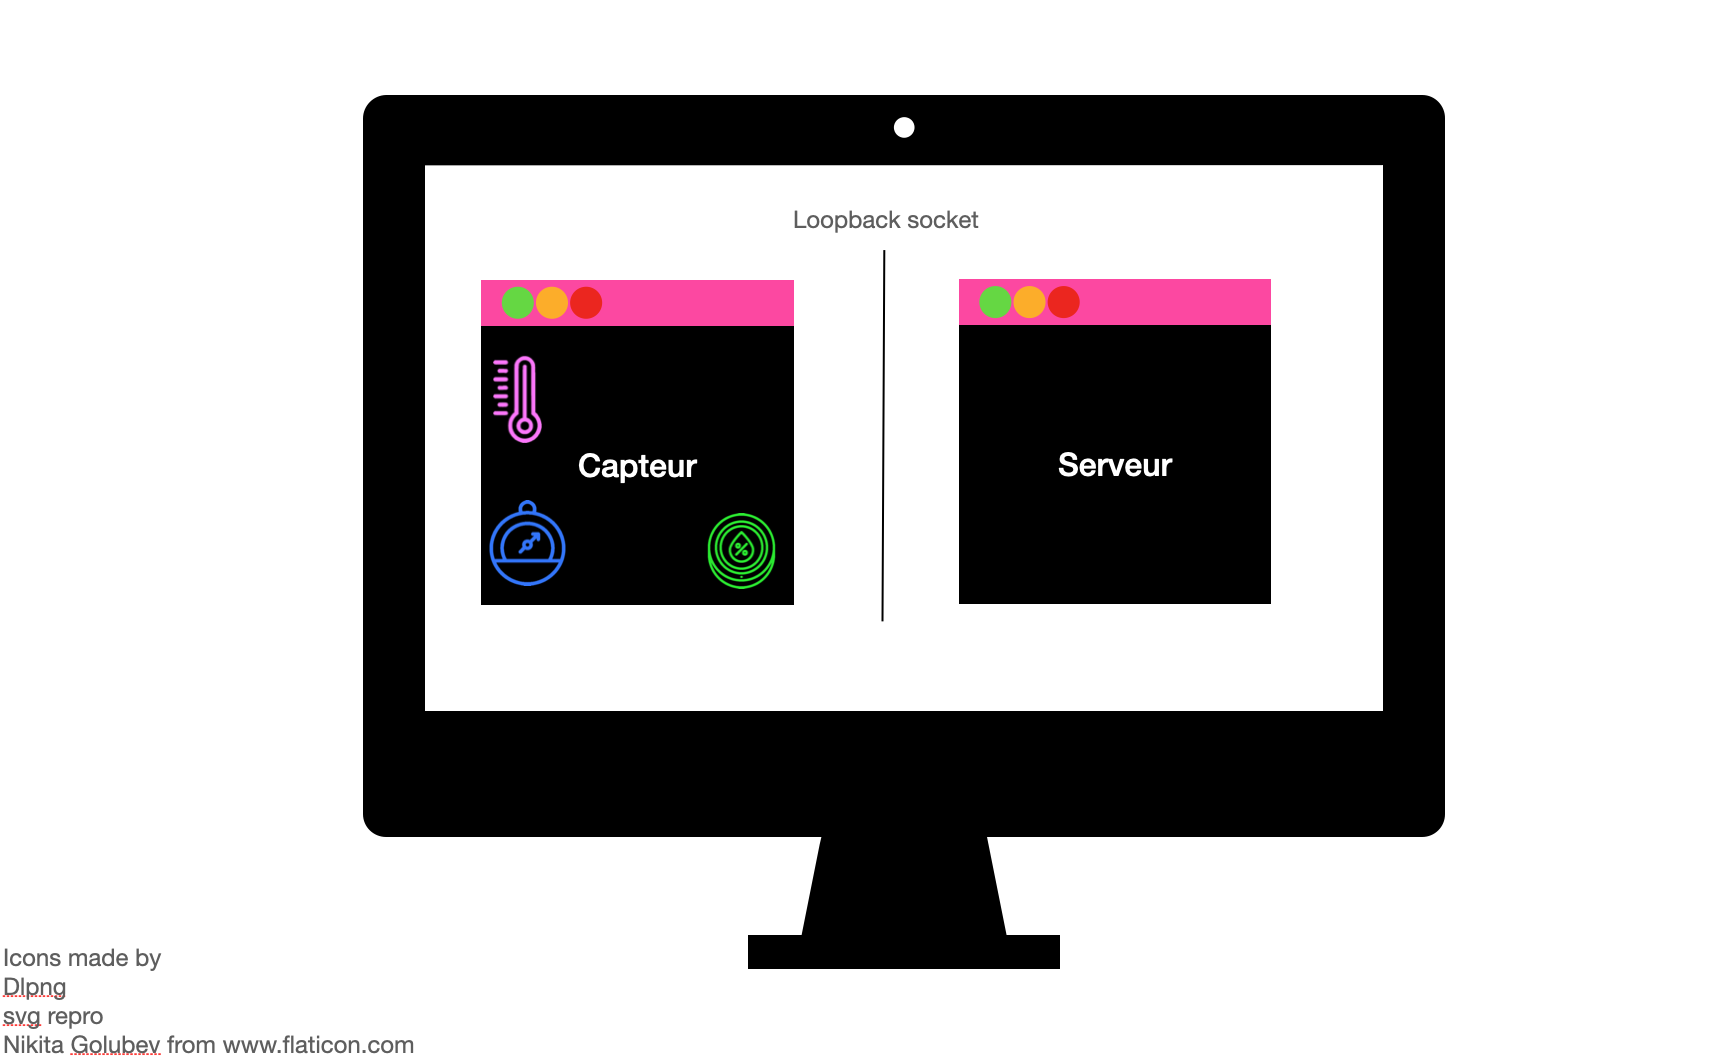
\includegraphics[width=1\columnwidth]{Pictures/Capture24.png}}
\caption{Architecture client serveur}
\label{fig-deux-terminaux}
\end{figure}

\subsection{Serveur Minimal}\label{chap-mini-serv}

\pythonlst{minimal\_server.py}


Commençons par construire un serveur sommaire (\texttt{minimal\_server.py}) qui va afficher tout ce qu'il reçoit. 
\begin{itemize}
    \item lignes 1 et 2 les modules \texttt{socket} pour la communication et \texttt{binascii} pour transformer le binaire en chaîne de caractères.
    \item ligne 4, la \pfunction{socket}{socket} crée la socket \texttt{s} avec les paramètres pour des communications IP (\texttt{AF\_INET}) et UDP (\texttt{SOCK\_DGRAM}).
    \item ligne 5, la socket est associée au numéro de port \texttt{33033} via la fonction \pfunction{socket}{bind}. L'adresse \texttt{0.0.0.0} indique que les données peuvent venir de n'importe quelle interface (Ethernet, Wi-Fi, loopback,...) 
    \item ligne 8, dans la boucle sans fin, la fonction \pfunction{socket}{recvfrom} va se bloquer dans l'attente de données. Elle retourne les données et l'adresse de l'émetteur.
    \item ligne 9, les données sont affichées en chaîne d'octets et en hexadécimal.
    
\end{itemize}

     \vspace{1em}

On lance le programme serveur. Comme personne lui parle, il n'affiche rien. 

\subsection{Capteur virtuel}

\pythonlst{virtual\_sensor.py}

Le module \Index{virtual\_sensor} avec la classe du même nom, reflète de manière à peu près réaliste le comportement d'un capteur. On voit dans le programme principal (ligne 23 à 37) que l'on créé trois capteurs virtuels : un pour la température (ligne 31), un autre pour la pression (ligne 32), et le troisième pour l'humidité (ligne 34). L'argument \texttt{start} précise la valeur de départ, \texttt{variation} la plage de variation entre deux mesures et \texttt{min} et \texttt{max} les valeurs à ne pas dépasser. La boucle sans fin qui affiche les différentes valeurs toutes les secondes.

\begin{termc}[backgroundcolor=\color{palerod}, language=json, basicstyle=\ttfamily\small, escapechar=@]
> @\textbf{python3 virtual\_sensor.py}@
 54.956    999.850  30.609
 54.963   1000.473  32.505
 55.062   1000.845  31.870
 55.017   1001.619  32.257
 55.083   1000.767  31.757
 55.027   1001.442  31.742
 \end{termc} 

\subsubsection{Envoi direct}

\pythonlst{minimal\_client1.py}
Des scripts utilisant ce module peuvent être écrit, comme par exemple le programme \texttt{minimal\_client1.py}.

La variable \texttt{t} contient la température qui est émise sur le port 33033 à l’adresse de \textit{loopback}. On obtient ainsi une communication entre deux programmes dans votre ordinateur dont l'adresse IP locale est \texttt{127.0.0.1}. Mais quand on lance le programme \texttt{minimal\_client1.py}, on obtient l’erreur suivante :

\begin{termc}[backgroundcolor=\color{palerod}, language=json, basicstyle=\ttfamily\small, escapechar=@]
 >python3.5 minimal_client1.py
Traceback (most recent call last):
  File "minimal_client1.py", line 11, in <module>
    s.sendto (t, ("127.0.0.1", 33033))
TypeError: a bytes-like object is required, not 'float'
\end{termc}

\Question{Bug ?}
{Pourquoi le programme client ne fonctionne pas ?
\begin{itemize}[label=$\circ$]
   \item \Wrong{L’adresse IP n’est pas correcte.}
   \item \Correct{Il manque un processus de sérialisation de la donné}
   \item \Wrong{La variable \texttt{t} n’est pas définie}
   \item \Wrong{La variable \texttt{t} ne peux pas être lue.}
 \end{itemize}
}
{La variable \texttt{t} pointe vers une représentation en mémoire du nombre flottant. Elle ne peut pas être directement envoyée à un autre équipement. Il faut ajouter une phase de sérialisation qui va permettre de transmettre cette information soit en une chaîne de caractères, soit en une chaîne d'octets.}

\subsubsection{Envoi d'une chaîne d'octets}

\pythonlst[firstline=9,lastline=11, firstnumber=9]{minimal\_client2.py}

Dans le programme \texttt{minimal\_client2.py}, le nombre flottant contenu dans la variable \texttt{t} est transformé en chaîne de caractères avec la fonction \texttt{\Index{str}}, puis en chaîne d'octets avec la méthode \pfunction{str}{encode} pour être compatible avec l'argument attendu par la méthode \pfunction{socket}{sendto}. Coté serveur la fonction \texttt{\Index{str}} converti la chaîne d'octets reçue en flottant.

\subsubsection{Envoi de plusieurs valeurs}

\pythonlst[firstline=11,lastline=17, firstnumber=11]{minimal\_client3.py} % 

Pour envoyer simultanément les valeurs des trois capteurs, la représentation via une chaîne de caractères est un peu plus compliquée à mettre en oeuvre. Si le programme \texttt{minimal\_client3.py} utilise \pfunction{str}{format} pour envoyer des données séparées par des vigules. Côté serveur, il faut décoder cette chaîne pour y retrouver les entiers. Et ça c'est beaucoup plus complexe à faire ! 

\subsubsection{JSON}

\pythonlst[firstline=12,lastline=19, firstnumber=12]{minimal\_client4.py} %

La solution la plus simple est de mettre ces trois valeurs dans un tableau python et de le transformer en une représentation JSON grâce à la fonction \pfunction{json}{dumps} du module \texttt{json}. 

     \vspace{1em}

Cette chaîne de caractères JSON est à son tour transformé en chaîne d'octets avec encode et envoyée au serveur. Dans notre cas, le serveur ne fait qu'afficher la chaîne de caractères mais vous pouvez utiliser la méthode \pfunction{json}{loads} du module \texttt{json} pour desérialiser et en faire une structure Python dans le serveur, sur laquelle il est maintenant facile d'effectuer des opérations comme, par exemple, un calcul de moyenne.

\begin{termc}[backgroundcolor=\color{palerod}, language=json, basicstyle=\ttfamily\tiny, escapechar=@]
% @\textbf{python3 minimal\_server.py}@
b'[19.93044784157464, 999.1552628155773, 35.723583473834566]' => b'5b31392e39333034343738343135373436342c203939392e313535c...
b'[19.940155545405723, 998.7581534530281, 35.820037116376184]' => b'5b31392e3934303135353534353430353732332c203939382e3735...
b'[20.003803212269627, 999.3517302791449, 34.33544522779677]' => b'5b32302e3030333830333231323236393632372c203939392e33353...
\end{termc}

\section{CBOR}

\begin{wrapfigure}{r}{3cm}
\Youtube{https://youtu.be/PmudahiRWFw}
\end{wrapfigure}

Le passage de JSON à CBOR est très simple. Il suffit de changer un module \texttt{cbor} à la place du module de \texttt{json}. Le programme \texttt{minimal\_client5.py}~:
\begin{itemize}
    \item ligne 1 fait appel au module cbor2 en le renommant cbor
    \item le reste du programme est identique au précédent, ce n'est que dans la la sérialisation, ligne 18, que la fonction \texttt{json.\pfunction{json}{dumps}} est remplacée par \texttt{cbor.\pfunction{cbor2}{dumps}}. Le format retourné étant une chaîne d'octets, il n'est plus nécessaire de faire appel à la méthode \texttt{encode}.
\end{itemize}


     \vspace{1em}


Le programme \pprog{minimal\_server.py} n'est pas modifié puisqu'il ne fait qu'afficher ce qu'il reçoit. 







\begin{termc}[backgroundcolor=\color{palerod}, language=json, basicstyle=\ttfamily\small, escapechar=#]
> #\texttbf{python3 minimal\_server.py}#
b'\x83... => b'83fb40341086f3e8b66bfb408f3b7791c8d61ffb403fac15ba06088e'
b'\x83... => b'83fb40341d4d28495268fb408f33d502185c3dfb403d95a2c4981444'
\end{termc}


\pythonlst{minimal\_client5.py}

On obtient le résultat suivant. La séquence CBOR fait 28 octets de long, l'équivalant JSON aurait fait 60 octets. Même si cela divise par deux la taille des données à transmettre, le résultat n'est pas compact. Cela tient à la représentation des nombres flottants en CBOR, car ici les flottant sont codés sur 8 octets.

\Question{Décodage}{
Analysons la séquence reçue: \texttt{83fb40341086f3e8b66bfb408f3b7791c8d61ffb403fac 15ba06088e}

À quoi correspond l’octet 0x83 qui commence la structure CBOR reçue ?
\begin{itemize}[label=$\circ$]
   \item \Wrong{au codage de l'entier positif 131 .}
   \item \Wrong{au codage de l'entier négatif 132 .}
   \item \Correct{à la définition d'un tableau de 3 éléments.́}
   \item \Wrong{à la définition d'un map CBOR de 3 éléments}
   \item \Wrong{à la définition d'un tableau de taille non définie.}
 \end{itemize}
 }
 {
 0x83 s'écrit en binaire \texttt{100-0 0111}. \texttt{100} est le type majeur pour un tableau. La valeur \texttt{00111} est inférieure à 24. Il s'agit donc du nombre d'éléments du tableau, donc un tableau de 3 éléments.
 }

\Question{Flottant}
{Dans cette chaîne, uel est le marqueur CBOR (en hexadécimal) qui indique que l’on a un nombre flottant ?}
{0xFB, si on l'écrit en binaire on obtient \texttt{111-1 1100}. Le majeur correspond à la catégorie des flottant et des valeurs spéciales.}

\Question{Taille du flottant}
{Quelle est la taille de ce flottant en octets ?}
{8 octets~; la partie mineur \texttt{1 1100} indique qu'il s'agit d'un flottant codé sur 8 octets}

\subsubsection{Utilisation de nombres entiers}

Pour réduire la taille des données transmises, nous allons utiliser des nombres entiers. Nous aurons besoin d’une précision au centième (deux chiffres après la virgule). Pour ce faire, il suffit, du coté du client, de prendre la partie entière du nombre multiplié par 100 et, du côté du serveur, de diviser la valeur reçue par 100. La modification du code est mineure.

\pythonlst[firstline=17,lastline=18, firstnumber=17]{minimal\_client6.py}


\begin{termc}[backgroundcolor=\color{palerod}, language=json, basicstyle=\ttfamily\tiny, escapechar=#]
> #\texttbf{python3 minimal\_server.py}#
b'\x83\x19\x07\xd7\x1a\x00\x01\x86O\x19\x0c\xa7' => b'831907d71a0001864f190ca7'
b'\x83\x19\x07\xd4\x1a\x00\x01\x86f\x19\x0cJ' => b'831907d41a00018666190c4a'
b'\x83\x19\x07\xd4\x1a\x00\x01\x86\x92\x19\rP' => b'831907d41a00018692190d50'
\end{termc}

La modification est mineure et tient en 12 octets, mais il y a une diminution au niveau de l'interopérabilité, car les deux entités doivent connaître la transformation de la valeur liée à la multiplication par 100.

\Question{Anticipons la taille}
{ Quelle est la taille minimale et maximale de la structure CBOR envoyée, en prenant en compte les valeurs possibles.
}
{
\begin{itemize}
    \item La température peut évoluer raisonnablement entre -30 et +50, soit -3000 et +5000 après la transformation en entier. La taille minimale, si on envoie 0, la taille sera d'un octet. La taille maximale tiennent sur 3 octets (1 pour le type/longueur et 2 pour les valeurs) 
    \item La pression évolue autour de 1000, soit 100~000 après la transformation en entier. La taille sera toujours de 5 octets (1 pour le type/longueur, 4 pour les valeurs)
    \item Le taux d'humidité évolue entre 0 et 100 , soit 0 et 10 000 après la transformation en entier. L a taille entre 1 octet et 3 octets
\end{itemize}

Si on ajoute le type/longueur 0x83 pour indiquer un tableau de trois éléments, on obtient une taille minimale de 1+1+5+1= 8 octets et une taille maximale de 1+3+5+3 = 12 octets.
}
